\documentclass[tikz]{standalone}
\usepackage{pgfplots}
\pgfplotsset{compat=1.15}
\usepackage{mathrsfs}
\usetikzlibrary{arrows,calc}
\usepackage{tkz-euclide}

\pagestyle{empty}

\definecolor{AngleClr}{rgb}{0,0.39215686274509803,0}
\definecolor{ShapeClr}{rgb}{0.6,0.2,0}
\definecolor{SecondAngleClr}{RGB}{14, 70, 161}

\begin{document}

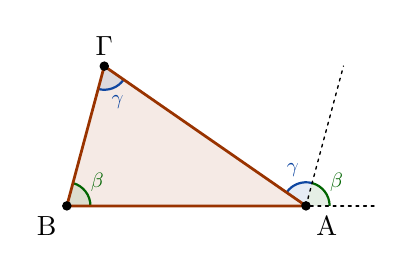
\begin{tikzpicture}[scale=.75]
\tkzSetUpLine[line width=1pt,color=black]
\tkzSetUpPoint[fill=black]

\tkzDefPoints{0/0/B,4.05/0/C}
\tkzDefPoint(75:2.45){A}

\tkzDefLine[parallel=through C](B,A) \tkzGetPoint{x}

\tkzDefPointOnLine[pos=1.2](A,B)\tkzGetPoint{A1}
\tkzDefPointOnLine[pos=-0.2](A,B)\tkzGetPoint{A2}
\tkzDefPointOnLine[pos=1.2](B,C)\tkzGetPoint{B1}
\tkzDefPointOnLine[pos=-0.2](B,C)\tkzGetPoint{B2}
\tkzDefPointOnLine[pos=1.2](C,A)\tkzGetPoint{C1}
\tkzDefPointOnLine[pos=-0.2](C,A)\tkzGetPoint{C2}


\tkzFillPolygon[fill=ShapeClr,fill opacity=0.1](A,B,C)

\tkzFillAngle[fill=AngleClr,size=.4,fill opacity=0.1](C,B,A)
\tkzMarkAngle[line width=0.8pt,size=.4,color=AngleClr](C,B,A)

\tkzFillAngle[fill=SecondAngleClr,size=.4,fill opacity=0.1](B,A,C)
\tkzMarkAngle[line width=0.8pt,size=.4,color=SecondAngleClr](B,A,C)

\tkzFillAngle[fill=SecondAngleClr,size=.4,fill opacity=0.1](x,C,A)
\tkzMarkAngle[line width=0.8pt,size=.4,color=SecondAngleClr](x,C,A)

\tkzFillAngle[fill=AngleClr,size=.4,fill opacity=0.1](B1,C,x)
\tkzMarkAngle[line width=0.8pt,size=.4,color=AngleClr](B1,C,x)

\tkzLabelAngle[pos=0.65](C,B,A){\scalebox{0.75}{\textcolor{AngleClr}{$\beta$}}}
\tkzLabelAngle[pos=0.65](B,A,C){\scalebox{0.75}{\textcolor{SecondAngleClr}{$\gamma$}}}

\tkzLabelAngle[pos=0.65](B1,C,x){\scalebox{0.75}{\textcolor{AngleClr}{$\beta$}}}
\tkzLabelAngle[pos=0.65](x,C,A){\scalebox{0.75}{\textcolor{SecondAngleClr}{$\gamma$}}}


\tkzDrawSegment[line width=0.5pt,color=black,dashed,dash pattern=on 1pt off 1.75pt,add=0 and 0.3](B,C)
\tkzDrawSegment[line width=0.5pt,color=black,dashed,dash pattern=on 1pt off 1.75pt](C,x)

\tkzDrawPolygon[color=ShapeClr](A,B,C)

\tkzDrawPoints[size=3](A,B,C)
\tkzLabelPoint[above](A){$\rm \Gamma$}
\tkzLabelPoint[below left](B){$\rm B$}
\tkzLabelPoint[below right](C){$\rm A$}


\end{tikzpicture}

\end{document}
